\begin{figure*}[t]
    \centering
    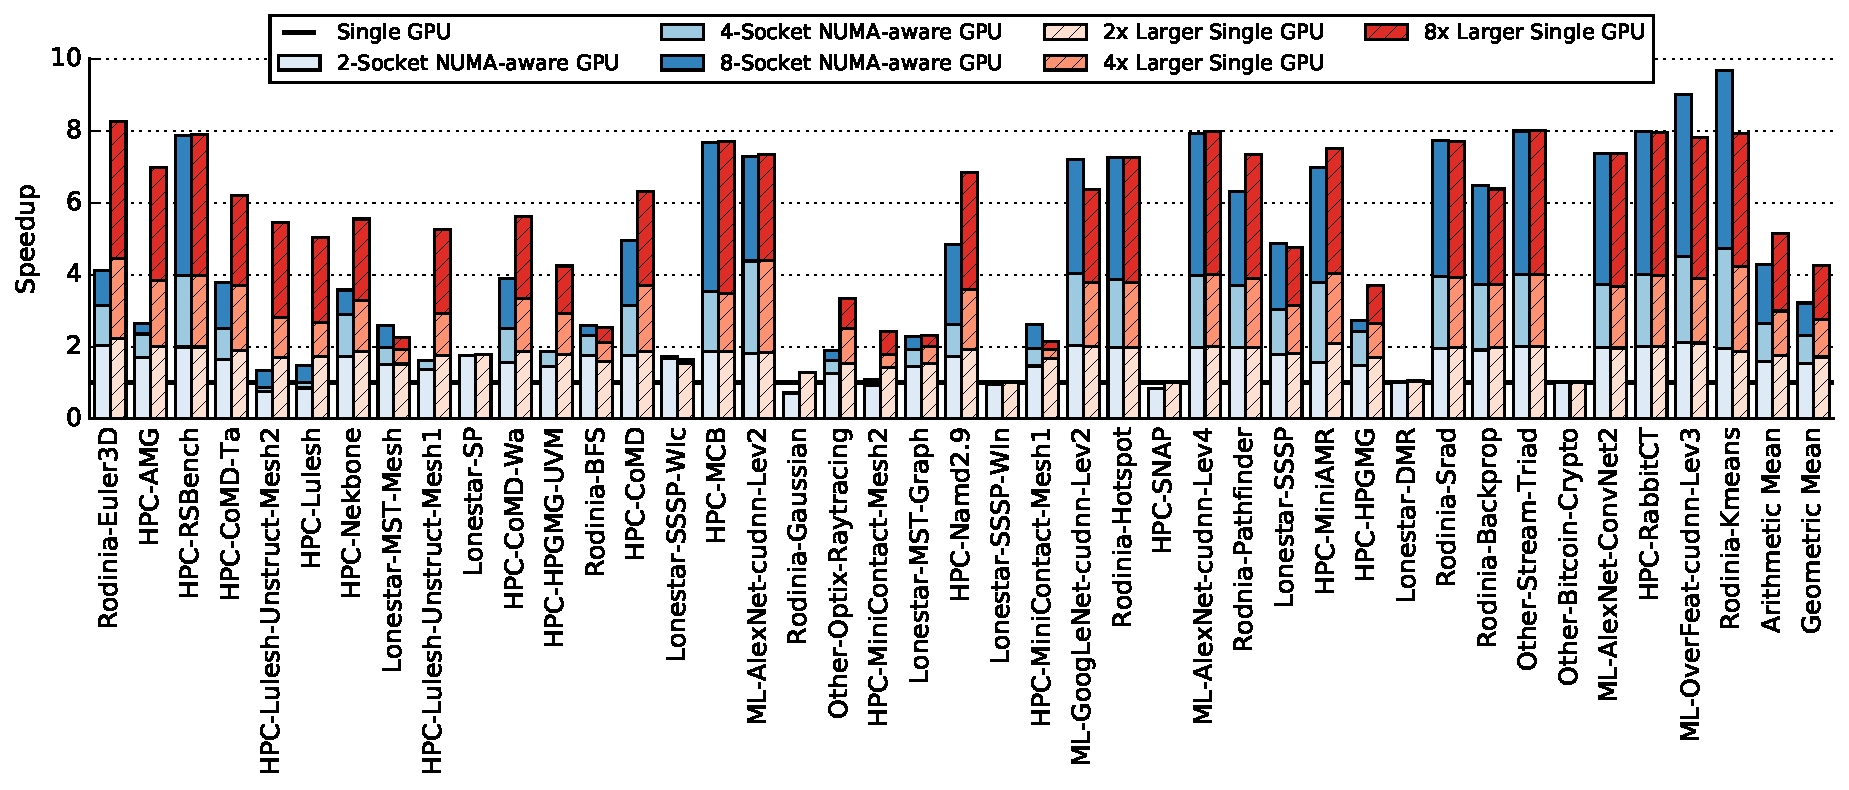
\includegraphics[width=1.0\textwidth]{figures/plot_scalability_mgpu_WB.pdf}
    \caption{Performance scalability of a NUMA-aware GPU compared to theoretical 
    maximum applications performance moving from 1 to 8 GPU sockets.}
    \label{fig:scalability}
    \vspace{-.2in}
\end{figure*}

\section {Discussion}
\label{sec:discussion}
\textbf{Combined Improvement:} Sections~\ref{sec:interconnect} 
and~\ref{caching} provide two techniques aimed at more efficiently utilizing 
scarce NUMA bandwidth within future NUMA multi-GPU system. These two 
techniques (interconnect balancing and NUMA-aware cashing) are orthogonal and 
can be applied in isolation or combination.  Dynamic interconnect balancing 
has an implementation advantage in that the system level changes to enable 
this feature are isolated from the larger GPU design.  Conversely, enabling 
GPU caching of both remote memory and dynamic balancing of cache capacity 
based on interconnect utilization requires changes to both the physical cache 
architectures and the GPU coherence protocol.

Because these two features target similar improvements, when employed 
together their effects are not strictly additive.  Figure~\ref{fig:combined} 
shows the improvement when applying both dynamic interconnects and NUMA-aware 
cache management together.  For benchmarks such as \texttt{CoMD}, these 
features contribute nearly equally to the overall improvement, but for others 
such as \texttt{ML-AlexNet-cudnn-Lev2} or \texttt{HPC-MST-Mesh1}, 
interconnect improvements or caching are the primary contributor 
respectively.  On average, we observe that when combined we see 2.13$\times$ improvement over single GPU and 73\% 
over the baseline software locality optimized 4-socket NUMA GPU 
using memory side L2 caches.

\textbf{Scalability:} Ultimately, for vendors to produce multi-socket NUMA 
GPUs they must scale efficiently enough for single application customers to 
see large enough performance improvements to justify their cost.  To 
understand the scalability of this approach Figure~\ref{fig:scalability} 
shows the performance of a NUMA-aware multi-socket GPU compared to a single 
GPU, when scaled across 2,4, and 8 sockets respectively.  On average a 2 
socket NUMA GPU achieves 53\% speedup, while 4 sockets and 8 sockets achieve 
2.33$\times$ and 3.27$\times$ speedup respectively.  Depending on customer expectations these 
speedups may look attractive or lackluster, particularly when per-benchmark 
variance is included.  However, the scalability of NUMA GPU's is not solely 
dependent on NUMA GPU microarchitecture. We observe that for some 
applications, even if the application was run on much larger hypothetical 
single GPUs, performance would not scale.  This may be due to a variety of 
reasons beyond NUMA effects, including number of CTA's available, expensive 
global synchronizations, or other factors.  Comparing our NUMA-aware GPU 
implementation to this hypothetical scaling that applications could achieve, 
we see that we can achieve 89\%, 84\%, and 75\% of overall application 
scalability at 2, 4, and 8 socket configurations respectively.  This good 
scaling factor indicates that the NUMA aspects of future multi-socket GPUs 
have largely been eliminated as performance limiters in single GPU 
application scaling via a NUMA-aware GPU design.

\textbf{Multi-Tenancy of Large GPUs:} In this work we have shown that many 
workloads today have the ability to saturate (with sufficient parallel work) 
a GPU that is at least 4$\times$ larger than today's GPUs.  With deep data 
becoming commonplace across many computing paradigms, we believe that the 
trend of having enough computation to saturate much larger single GPUs will 
continue into the foreseeable future. However, when GPUs become larger at the 
expense of having multiple discrete GPUs within the system, questions related 
to GPU provisioning arise.  Applications that cannot saturate such a GPU will 
leave resources underutilized and applications that may be running 
concurrently in the system currently have to coarse grain multiplex the GPU 
in time cooperatively. 

While not the focus of this work, there is significant effort in both 
industry and academia to support finer grain sharing of GPUs through either 
shared SM execution~\cite{tanasic2014enabling}, spatial multiplexing of a 
GPU~\cite{park2015chimera}, or through improved time division multiplexing 
with GPU pre-emptability~\cite{lin2016enabling}.  To support improved per GPU 
efficiency, any of these solutions could be applied to a multi-socket GPU to 
improve utilization in cases where applications can not fill a significantly 
larger GPU.  Alternatively, with additional software work multi-socket GPU 
designs should be able to be dynamically partitioned with granularity from 
1--N logical GPUs if they are switch connected, providing yet another level 
of flexibility.

\textbf{Power Implications:} As discussed, arbitrarily large monolithic 
single GPUs are unfeasible, so discrete Multi-GPUs connected with on board 
high-speed links and switches become an attractive solution for continuing 
performance scaling. However, these on board high-speed links and switches 
require additional power. We estimated such overheads by assuming $10 pJ/b$ of 
on board interconnect energy for combined links and switch (extrapolated from 
publicly available information for cabinet level Mellanox switches and 
links~\cite{mlswitch,mlnic}). By using this estimate we calculated an average 
$79 W$ (Geo-Mean $30 W$) of communication power for the baseline 
architecture composed of 4 GPUs, and of $50 W$ (Geo-Mean $14 W$) after 
our optimizations are applied. Some applications such as 
\texttt{Rodinia-Euler3D, HPC-Lulesh, HPC-AMG, HPC-Lulesh-Unstruct-Mesh2} are 
quite demanding in terms of communication, resulting in $\approx 200 W$ 
of communication power for the baseline and $\approx 130 W$ after our 
optimizations are considered. Assuming a typical TDP of $250 W$ per GPUs, 
in a 4 GPUs system, the extra power due to the communication represents in 
average $8\%$ for the baseline and $5\%$ after our optimization are applied 
for the 41 considered benchmarks.
